\documentclass[journal,12pt,twocolumn]{IEEEtran}

\usepackage{setspace}
\usepackage{gensymb}

\singlespacing


\usepackage[cmex10]{amsmath}

\usepackage{amsthm}

\usepackage{mathrsfs}
\usepackage{txfonts}
\usepackage{stfloats}
\usepackage{bm}
\usepackage{cite}
\usepackage{cases}
\usepackage{subfig}

\usepackage{longtable}
\usepackage{multirow}

\usepackage{enumitem}
\usepackage{mathtools}
\usepackage{steinmetz}
\usepackage{tikz}
\usepackage{circuitikz}
\usepackage{verbatim}
\usepackage{tfrupee}
\usepackage[breaklinks=true]{hyperref}
\usepackage{graphicx}
\usepackage{tkz-euclide}

\usetikzlibrary{calc,math}
\usepackage{listings}
    \usepackage{color}                                            %%
    \usepackage{array}                                            %%
    \usepackage{longtable}                                        %%
    \usepackage{calc}                                             %%
    \usepackage{multirow}                                         %%
    \usepackage{hhline}                                           %%
    \usepackage{ifthen}                                           %%
    \usepackage{lscape}     
\usepackage{multicol}
\usepackage{chngcntr}

\DeclareMathOperator*{\Res}{Res}

\renewcommand\thesection{\arabic{section}}
\renewcommand\thesubsection{\thesection.\arabic{subsection}}
\renewcommand\thesubsubsection{\thesubsection.\arabic{subsubsection}}

\renewcommand\thesectiondis{\arabic{section}}
\renewcommand\thesubsectiondis{\thesectiondis.\arabic{subsection}}
\renewcommand\thesubsubsectiondis{\thesubsectiondis.\arabic{subsubsection}}


\hyphenation{op-tical net-works semi-conduc-tor}
\def\inputGnumericTable{}                                 %%

\lstset{
%language=C,
frame=single, 
breaklines=true,
columns=fullflexible
}
\begin{document}


\newtheorem{theorem}{Theorem}[section]
\newtheorem{problem}{Problem}
\newtheorem{proposition}{Proposition}[section]
\newtheorem{lemma}{Lemma}[section]
\newtheorem{corollary}[theorem]{Corollary}
\newtheorem{example}{Example}[section]
\newtheorem{definition}[problem]{Definition}

\newcommand{\BEQA}{\begin{eqnarray}}
\newcommand{\EEQA}{\end{eqnarray}}
\newcommand{\define}{\stackrel{\triangle}{=}}
\bibliographystyle{IEEEtran}

\providecommand{\mbf}{\mathbf}
\providecommand{\pr}[1]{\ensuremath{\Pr\left(#1\right)}}
\providecommand{\qfunc}[1]{\ensuremath{Q\left(#1\right)}}
\providecommand{\sbrak}[1]{\ensuremath{{}\left[#1\right]}}
\providecommand{\lsbrak}[1]{\ensuremath{{}\left[#1\right.}}
\providecommand{\rsbrak}[1]{\ensuremath{{}\left.#1\right]}}
\providecommand{\brak}[1]{\ensuremath{\left(#1\right)}}
\providecommand{\lbrak}[1]{\ensuremath{\left(#1\right.}}
\providecommand{\rbrak}[1]{\ensuremath{\left.#1\right)}}
\providecommand{\cbrak}[1]{\ensuremath{\left\{#1\right\}}}
\providecommand{\lcbrak}[1]{\ensuremath{\left\{#1\right.}}
\providecommand{\rcbrak}[1]{\ensuremath{\left.#1\right\}}}
\theoremstyle{remark}
\newtheorem{rem}{Remark}
\newcommand{\sgn}{\mathop{\mathrm{sgn}}}
\providecommand{\abs}[1]{\left\vert#1\right\vert}
\providecommand{\res}[1]{\Res\displaylimits_{#1}} 
\providecommand{\norm}[1]{\left\lVert#1\right\rVert}
%\providecommand{\norm}[1]{\lVert#1\rVert}
\providecommand{\mtx}[1]{\mathbf{#1}}
\providecommand{\mean}[1]{E\left[ #1 \right]}
\providecommand{\fourier}{\overset{\mathcal{F}}{ \rightleftharpoons}}
%\providecommand{\hilbert}{\overset{\mathcal{H}}{ \rightleftharpoons}}
\providecommand{\system}{\overset{\mathcal{H}}{ \longleftrightarrow}}
	%\newcommand{\solution}[2]{\textbf{Solution:}{#1}}
\newcommand{\solution}{\noindent \textbf{Solution: }}
\newcommand{\cosec}{\,\text{cosec}\,}
\providecommand{\dec}[2]{\ensuremath{\overset{#1}{\underset{#2}{\gtrless}}}}
\newcommand{\myvec}[1]{\ensuremath{\begin{pmatrix}#1\end{pmatrix}}}
\newcommand{\mydet}[1]{\ensuremath{\begin{vmatrix}#1\end{vmatrix}}}
\numberwithin{equation}{subsection}

\makeatletter
\@addtoreset{figure}{problem}
\makeatother
\let\StandardTheFigure\thefigure
\let\vec\mathbf

\renewcommand{\thefigure}{\theproblem}

\def\putbox#1#2#3{\makebox[0in][l]{\makebox[#1][l]{}\raisebox{\baselineskip}[0in][0in]{\raisebox{#2}[0in][0in]{#3}}}}
     \def\rightbox#1{\makebox[0in][r]{#1}}
     \def\centbox#1{\makebox[0in]{#1}}
     \def\topbox#1{\raisebox{-\baselineskip}[0in][0in]{#1}}
     \def\midbox#1{\raisebox{-0.5\baselineskip}[0in][0in]{#1}}
\vspace{3cm}
\title{Assignment 5}
\author{Sachinkumar Dubey - EE20MTECH11009}

\maketitle
\newpage
\bigskip
\renewcommand{\thefigure}{\theenumi}
\renewcommand{\thetable}{\theenumi}
Download all python codes from 
\begin{lstlisting}
https://github.com/sachinomdubey/Matrix-theory/Assignment5/codes
\end{lstlisting}
%
and latex-tikz codes from 
%
\begin{lstlisting}
https://github.com/sachinomdubey/Matrix-theory/Assignment5
\end{lstlisting}
\subsection{Problem}
(Geolin 1.9) $AB$ is a line-segment. $P$ and $Q$ are points on opposite sides of $AB$ such that each of them is equidistant from the points $A$ and $B$. Show that the line $PQ $ is the perpendicular bisector of $AB$.
\begin{figure}[h!]
\centering
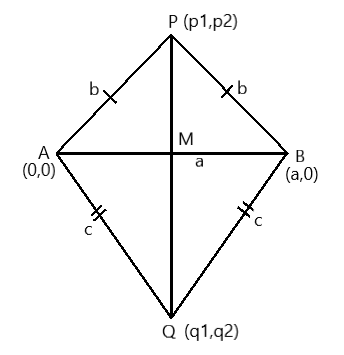
\includegraphics[width=7cm, height=7cm]{Figure_51}
\caption{}
\label{Fig4}
\end{figure}
\subsection{Explanation}
In order to prove that line $PQ $ is the perpendicular bisector of $AB$, two conditions need to be met:
\begin{enumerate}
    \item Angle between line $AB$ and line $PQ$ should be $90\degree$.
    \item $AM$=$BM$
\end{enumerate}
Steps to prove the first condition are as follow:
\begin{enumerate}
    \item Here, the following information is given:
    \begin{align}
    \norm{\vec{P}-\vec{A}}=\norm{\vec{P}-\vec{B}} \label{eq2.2}\\
    \norm{\vec{Q}-\vec{A}}=\norm{\vec{Q}-\vec{B}}
\end{align}
    \item Take the norms and simplify to get $\vec{P}$ and $\vec{Q}$. Using $\vec{P}$ and $\vec{Q}$, prove the following condition to show that lines $PQ$ is the perpendicular to line $AB$:
    \begin{align}
    \myvec{\vec{P}-\vec{Q}}^T\myvec{\vec{A}-\vec{B}}=0
    \end{align}
\end{enumerate}
Steps to prove the second condition are as follow:
\begin{enumerate}
    \item Finding the normal vectors of line $PQ$. Further using the normal vector to find the equation of line $PQ$. 
    \item The solution of equation of line $AB$ and line $PQ$ will give the co-ordinates of point $M$. 
    \item Using the distance formula to prove that $AM$=$BM$.
\end{enumerate}
\subsection{Solution}
Let the Points $\vec{A}$, $\vec{B}$, $\vec{P}$ and $\vec{Q}$ be:
\begin{align}
    \vec{A}=\myvec{0 \\ 0} & \vec{B}=\myvec{a \\ 0} & \vec{P}=\myvec{p_1 \\ p_2}&\vec{Q}=\myvec{q_1 \\ q_2}
\end{align}
The points $\vec{P}$ and $\vec{Q}$  are equidistant from the points $\vec{A}$ and $\vec{B}$. Then we can write:
\begin{align}
    \norm{\vec{P}-\vec{A}}=\norm{\vec{P}-\vec{B}} \label{eq2.2}\\
    \norm{\vec{Q}-\vec{A}}=\norm{\vec{Q}-\vec{B}} \label{eq2.3}
\end{align}
The equation \ref{eq2.2} can be further written as:
\begin{align}
    \norm{\myvec{p_1\\p_2}-\myvec{0\\0}}=\norm{\myvec{p_1\\p_2}-\myvec{a\\0}} \\
    \sqrt{p_1^2+p_2^2}=  \sqrt{(p_1-a)^2+p_2^2}\\
    p_1^2+p_2^2= p_1^2+p_2^2-2ap_1+a^2\\
    \therefore a^2-2ap_1=0\\
    \implies p_1=a/2\\
    \therefore \vec{P}=\myvec{a/2 \\ p_2}  \label{eq3.9}
\end{align}
Similarly, the equation \ref{eq2.3} can be further written as:
\begin{align}
    \norm{\myvec{q_1\\q_2}-\myvec{0\\0}}=\norm{\myvec{q_1\\q_2}-\myvec{a\\0}} \\
    \sqrt{q_1^2+q_2^2}=  \sqrt{(q_1-a)^2+q_2^2}\\
    q_1^2+q_2^2= q_1^2+q_2^2-2aq_1+a^2 \\
    \therefore a^2-2aq_1=0\\
    \implies q_1=a/2\\
    \therefore \vec{Q}=\myvec{a/2 \\ q_2} \label{eq3.15}
\end{align}
The lines $AB$ and $PQ$ will be perpendicular, when the following condition is met:
\begin{align}
    \myvec{\vec{P}-\vec{Q}}^T\myvec{\vec{A}-\vec{B}}=0\label{eq3.16}
\end{align}
Using equation \ref{eq3.9} and \ref{eq3.15}, The RHS can be written as:
\begin{align}
  RHS=\myvec{0 \\ (p_2-q_2)}^T\myvec{-a \\ 0}\\
  RHS=\myvec{0 & (p_2-q_2)}\myvec{-a \\ 0}\\
  RHS = 0\\
  \therefore RHS=LHS
\end{align}
Therefore, The lines $AB$ and $PQ$ are perpendicular to each other as the equation \ref{eq3.16} is satisfied. \\
The vector equations of lines $AB$ and $PQ$ can be written as:
\begin{align}
\vec{x}=\myvec{0\\0}+ \lambda_1 \myvec{-a \\ 0}\label{eq3.21}\\
\vec{x}=\myvec{a/2\\p_2}+ \lambda_2 \myvec{0 \\ (p_2-q_2)} \label{eq3.22}
\end{align}
The lines intersect at point M, Equating equations \ref{eq3.21} and \ref{eq3.22} and solving the equations in matrix form:
\begin{align}
-a\lambda_1=a/2\\
0= p_2+ \lambda_2 (p_2-q_2)\\
\myvec{-a & 0 &\vrule & a/2\\0 & (p_2-q_2) &\vrule& -p_2}\\
\xleftrightarrow[]{R_1\leftarrow R_1/-a}
\myvec{1 & 0 &\vrule & -1/2\\0 & (p_2-q_2) &\vrule& -p_2}\\
\xleftrightarrow[]{R_2\leftarrow R_2/(p_2-q_2)}
\myvec{1 & 0 &\vrule & -1/2\\0 & 1 &\vrule& -p_2/(p_2-q_2)}
\end{align}
Therfore, $\lambda_1 = -1/2$ and $\lambda_2=-p_2/(p_2-q_2)$\\
Putting these values in equation \ref{eq3.21}, We get point \vec{M} as:
\begin{align}
\vec{M}=\myvec{a/2\\0}
\end{align}
The segments $AM$ and $BM$ are given as:
\begin{align}
    AM=\norm{\vec{A}-\vec{M}} \\
    \therefore AM=\norm{\myvec{0\\0}-\myvec{a/2\\0}}\\
    \therefore AM=\sqrt{a^2/4+0}=a/2 \label{eq3.30}\\
    Similarly,BM=\norm{\vec{B}-\vec{M}} \\
    \therefore BM=\norm{\myvec{a\\0}-\myvec{a/2\\0}}\\
    \therefore BM=\sqrt{a^2/4+0}=a/2\label{eq3.33}
\end{align}
From equation \ref{eq3.30} and \ref{eq3.33} :
\begin{align}
    AM=BM \label{eq3.35}
\end{align}
Thus, Both conditions are satisfied, which make line $PQ$ perpendicular bisector of $AB$. Hence proved.
\end{document}